\PassOptionsToPackage{hyphens}{url}% allow line breaks at hyphens in urls
\documentclass[12pt]{matlatex}
\usepackage{examples}
\usepackage{pgfplots}
\usepackage{caption}

\begin{document}

\section*{Plotting Bessel functions}

This simple example uses Matlab to produce a plot of the first six Bessel functions. Two plots are shown, one created by Matlab and a second created by LaTeX using the plotting package {\tt\small pgfplots} and the data exported from Matlab.

This example is based upon the Mathworks example at%
\ \url{https://au.mathworks.com/matlabcentral/fileexchange/35229-matlab-plot-gallery-standard-line-colors}.


\begin{matlab}
   x  = 0:0.1:15;
   y0 = besselj(0,x);
   y1 = besselj(1,x);
   y2 = besselj(2,x);
   y3 = besselj(3,x);
   y4 = besselj(4,x);
   y5 = besselj(5,x);

   plot(x, y0, 'r', x, y1, 'g', x, y2, 'b',  ...
        x, y3, 'c', x, y4, 'm', x, y5, 'y');
   legend('J_0','J_1','J_2','J_3','J_4','J_5');

   print(gcf,'example_04_fig.png','-dpng');

   % Note: using ' on [x;y0...]' ensures the six functions are written as columns of example_01.txt

   dlmwrite ('example_04.txt',[x;y0;y1;y2;y3;y4;y5]','delimiter',' ','precision','% .8e');

\end{matlab}

\clearpage

\begin{figure}
   \centering
   \IfFileExists{example_04_fig.png}%
   {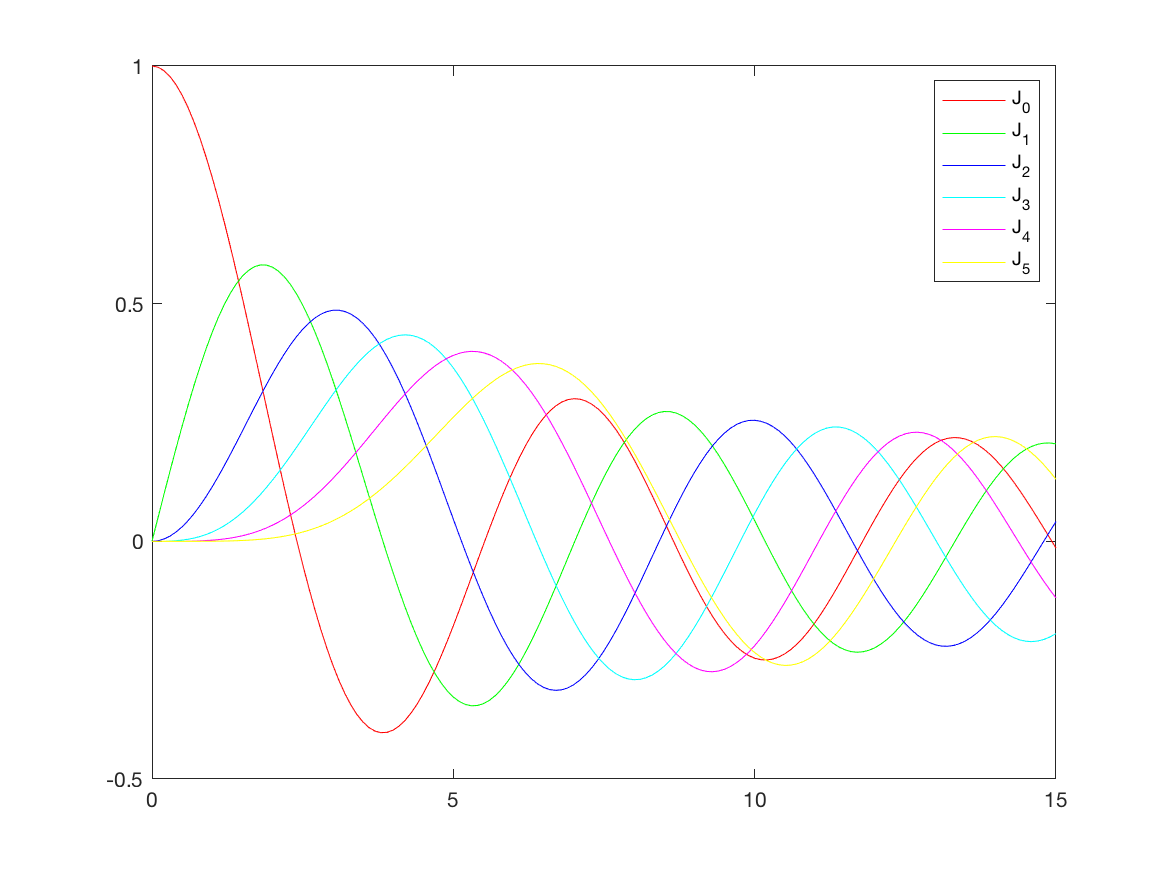
\includegraphics[width=6.4in]{example_04_fig.png}}{Failed to create png plot.}
   \caption{The first six Bessel functions.}
\end{figure}

\clearpage

\pgfplotsset{compat=newest}
\pgfplotsset{width=0.45\textwidth,height=0.34\textwidth}

\subsection*{Using pgfplots}

\begin{minipage}[t]{\textwidth}
   \centering
   \begin{tikzpicture}
      \begin{axis}
         [xmin= 0.0,  xmax=15.0,
          ymin=-0.45, ymax=1.05,
          xlabel=$x$, ylabel=$J_n(x)$,
          grid=major, grid style={dashed,gray!30},
          legend entries = {$J_0$, $J_1$, $J_2$, $J_3$, $J_4$, $J_5$}]
          \addplot[blue]   table [x index=0, y index=1]{example_04.txt};
          \addplot[red]    table [x index=0, y index=2]{example_04.txt};
          \addplot[green]  table [x index=0, y index=3]{example_04.txt};
          \addplot[teal]   table [x index=0, y index=4]{example_04.txt};
          \addplot[orange] table [x index=0, y index=5]{example_04.txt};
          \addplot[purple] table [x index=0, y index=6]{example_04.txt};
      \end{axis}
   \end{tikzpicture}
   \captionof{figure}{The first six Bessel functions.}
\end{minipage}

\vfill

\begin{latex}
   \begin{tikzpicture} % requires \usepackage{pgfplots}
      \begin{axis}
         [xmin= 0.0,  xmax=15.0,
          ymin=-0.45, ymax=1.05,
          xlabel=$x$, ylabel=$J_n(x)$,
          grid=major, grid style={dashed,gray!30},
          legend entries = {$J_0$, $J_1$, $J_2$, $J_3$, $J_4$, $J_5$}]
          \addplot[blue]   table [x index=0, y index=1]{example_04.txt};
          \addplot[red]    table [x index=0, y index=2]{example_04.txt};
          \addplot[green]  table [x index=0, y index=3]{example_04.txt};
          \addplot[teal]   table [x index=0, y index=4]{example_04.txt};
          \addplot[orange] table [x index=0, y index=5]{example_04.txt};
          \addplot[purple] table [x index=0, y index=6]{example_04.txt};
      \end{axis}
   \end{tikzpicture}
   \captionof{figure}{The first six Bessel functions.} % requires \usepackage{caption}
\end{latex}

\end{document}
